	La fin de la phase de développement approchant, l’équipe avait fait ressentir le besoin de procéder à la réalisation de tests de charge afin de vérifier la capacité des APIs à soutenir le trafic attendu. Pour cela, l’un des outils open source les plus performant et rapide à mettre en place du marché est \textbf{Apache JMeter} \cite{bib_jmeter}. Ainsi, afin de centraliser tous les tests et de gagner du temps sur la formation aux outils et leur installation, j’ai décidé d’utiliser JMeter pour aussi automatiser les tests fonctionnels. \\
	
	Ce logiciel, développé en java avec l’API Swing par la fondation Apache, permet de réaliser aussi bien des tests de performance que de charge ou encore fonctionnel compatibles avec un grand nombre de protocoles et technologies. Il permet de créer des requêtes et de les exécuter de manière automatique sur des serveurs web, des base de données via JDBC, sur des LDAP et bien d’autres. Celui-ci exporte le résultat des tests au format XML ce qui permet aisément de les réimporter sous TestLink. En effet, ce dernier nous offre la possibilité d’importer les résultats de tests via des fichiers aussi au format XML. Ainsi, il était possible de jouer les tests automatiquement dans un premier temps sur JMeter puis de générer, dans un second temps,  un rapport à destination du client via TestLink. En outre, JMeter met à notre disposition de nombreux avantages : \\
	
\begin{itemize}
	\item Logiciel open source disponible gratuitement
	\item Interface en Swing très intuitive
	\item Multithreading permettant de simuler la concurrence des requêtes lors des tests de charges via la mise en place de différents groupes de threads représentant des utilisateurs fictifs
	\item Possibilité d’installer de nombreux plugins développés par une communauté active afin de customiser les tests si besoin est \\
\end{itemize}
 
	Il propose de construire les plans de tests de manière interactive en ayant recours à des composants préconçus qui interagiront entre eux. Il en existe différents types pouvant être utilisés comme nous le montre le tableau figure \ref{composantJMeter} : \\

\begin{table}[h!]
	\center
	\begin{tabular}{| c | c |}
     \hline
     Composant & Description \\ \hline
     Moteur d’utilisateurs & Il s’agit de l’élément qui définira le niveau de la charge à appliquer \\ & (nombre d’utilisateurs, d’itération, temps de montée en charge) \\ \hline
     Contrôleur logique & Permet de structurer les tests \\ \hline
     Configuration & Permet de définir les configurations communes à plusieurs éléments \\ \hline
     Compteur de temps & Permet de gérer le temps d’attente avant l’exécution d’un composant \\ \hline
     Echantillons & Réalise les opérations de tests (ici des requêtes HTTP) \\ \hline
     Pré-processeurs & Agi avant les échantillons pour réaliser des opérations \\ \hline
     Post-processeurs & Agi sur le résultat des échantillons \\ \hline
     Récepteurs & Traite et formatent le résultat des tests \\ \hline
     Assertions & Permet de vérifier le résultat des échantillons \\ \hline
	\end{tabular}
	\caption{Composants JMeter}
	\label{composantJMeter}
\end{table}
	
	Les tests étant nombreux, j’ai décidé de les classer par service afin de rapidement en retrouver un en particulier et de pouvoir les jouer selon le microservice désiré. Cela s'est avéré utile par la suite, lorsqu'un service était défaillant, pour pouvoir facilement lancer les tests le concernant, étudier les réponses obtenues et cibler l'origine des anomalies. Il était, en effet, beaucoup plus rapide d'avoir recours à JMeter qui permettait d'envoyer de nombreuses requêtes avec différents paramètres plutôt que d'exécuter des requêtes manuellement via Postman jusqu'à réussir à reproduire un bug pour l'analyser. 
	
	Après cela, j’ai défini la structure du plan de test général qui devait contenir tous les tests fonctionnels en choisissant les composants qui allaient le constituer puis en procédant au paramétrage des différents éléments de configuration. La capture d’écran de JMeter figure \ref{jmeterPlanTest} montre la structure que j’ai établi pour le plan de test final et chacun des services. Cette structure est explicitée sous cette figure via une explication du détail de chaque élément employé ainsi que ses interactions avec les autres. \\
	
	\begin{figure}[h!]
		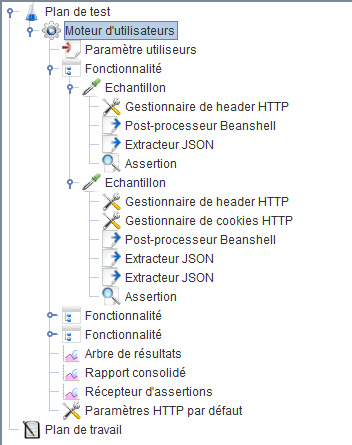
\includegraphics[scale=0.7]{images/travailNeuflizeOBC/testsFonc/jmeterPlanTest.png}
		\centering
		\caption{Plan de test JMeter}
		\label{jmeterPlanTest}
	\end{figure}
	
	\paragraph{1 - Moteur d'utilisateurs}
	Le moteur d'utilisateurs est l'élément englobant tous les composants, permettant de définir le niveau de charge affecté au plan de tests. Dans notre cas, ces derniers étant fonctionnels, le nombre de threads (utilisateurs) ainsi que le nombre d'itération des requêtes est de 1. De plus, le temps de montée en charge est laissé par défaut afin que les tests soient exécutés dans les meilleures conditions possibles.

	\paragraph{2 - Contrôleur logique}
	Les contrôleurs logiques permettent de définir la structure du plan de tests. Ici, il y en a un par service testé. Ils contiennent tous les tests d'un service particulier, les opérations à effectuer pour les mener à bien et les assertions.
	
	Par exemple, il y a le controleur NewTransfer regroupant les tests du service du même nom permettant de réaliser des transactions bancaires.
	
	\paragraph{2.1 - Echantillon}
	Les échantillons représentent les requêtes HTTP qui seront exécutées par JMeter. Afin de maintenir la cohérence avec TestLink, toutes les requêtes testées portent un nom de la forme NOBC-API-XX, ce qui correspond aux ID des cas de tests défini dans TestLink. Celles-ci sont alors vérifiées grâce à des assertions. Celles dont le nom n'est pas de cette forme ne sont pas vérifiées et n'ont pas d'assertions, elles ne sont exécutées que pour remplir les préconditions nécessaires à l'exécution des tests.
	
	Par exemple, pour pouvoir appeler le service NewTransfer, il faut l'identifiant d'un compte débiteur et créditeur, et comme pour tout service il faut un token d'authentification. Ainsi, il faut donc au minimum appeler les services AccountToDebit, Addessbook et TokenInfo, extraire les informations souhaitées puis les utiliser en paramètre de la requête vers NewTransfer.
	
	De manière générale, toutes les requêtes testées seront toujours au minimum précédée d'une requête de précondition permettant de générer le token d'authentification. Il s'agit de la raison majeure pour laquelle JMeter a permi un gain de temps considérable, il n'y avait en effet plus à se soucier d'aller chercher un token en passant par le TSE à chaque exécution de requête.
	
	\paragraph{2.2 - Json extractor}
	Cet élément est de type post-processeur et permet d'extraire la valeur d'un champ d'une réponse au format JSON en utilisant JsonPath, un langage permettant d'adresser une partie d'un document JSON, puis de la stocker dans une variable globale. Positionné dans un échantillon de type précondition, il permet d'extraire une information qui pourra ensuite être passée en paramètre d'une requpete testée.
	
	Par exemple, après l'appel à AccountToDebit, il permet de récupérer l'identifiant d'un compte débiteur qui sera utilisé comme paramètre dans la requête NOBC-API-28 vers NewTransfer.
	
	Cet élément est aussi utilisé sur les requêtes testées pour extraire les valeurs de tous les champs de la réponse afin qu'ils soient ensuite vérifiés par le biais d'assertions.
	
	\paragraph{2.3 - Beanshell extractor}
	Cet élément a le même objectif que json extractor mais utilise un script Beanshell à la place de JsonPath. Beanshell est un langage de script dont la syntaxe est très proche de Java, interprété et dynamiquement typé. JsonPath permet d'accéder à un champ JSON particulier mais ne permet pas de stipuler des conditions complexes, c'est pourquoi dans certains cas j'ai dû recourir à des scripts Beanshell pour récupérer une valeur bien précise dans un champ d'une réponse.
	
	Par exemple, supposons maintenant que l'on souhaite appeler le service NewTransfer. Il faut dans un premier temps récupérer l'id d'un compte débiteur via un appel à AccountToDebit, ce qui est faisable facilement via JsonPath. Ensuite, il faut récupérer un compte créditeur via un appel à AddressBook. Or, le compte créditeur doit obligatoirement être différent du compte débiteur, condition qu'il n'est pas possible de préciser via JsonPath, c'est pourquoi il faut recourir ici à un script Beanshell pour récupérer une valeur cohérente.
	
	\paragraph{2.4 - Assertion}
	Les éléments assertions sont aussi de type post-processeur et sont des scripts Beanshell dont l'objectif est de vérifier des conditions puis de retourner une réponse qui déterminera le status du test après son exécution (succès ou échec). Lorsque la requête à tester est exécutée, les éléments json extractor stockent les valeurs des champs de la réponse dans des variables qui pourront ensuite être utilisées dans ces scripts. Il ne reste plus qu'à écrire le script et les conditions de son succès/échec.
	
	\paragraph{2.5 - HTTP cookie manager}
	Elément de type pré-processeur permettant de configurer les cookies d'une requête avant son exécution. Ici, chaque requête doit au minimum posséder un cookie contenant le token d'authentification qui est récupéré automatiquement au préalable via l'exécution d'une requête permettant de générer ce dernier.
	
	\paragraph{2.6 - HTTP header manager}
	Elément de type pré-processeur permettant de configurer le header de la requête si besoin est. (par exemple le content-type)
	
	\paragraph{3 - View result tree}
	Elément permettant d'afficher, entre autre, le résultat de l'exécution de toutes les requêtes (succès/échec) ainsi que leur réponse. Celui-ci permet aussi de spécifier si l'on souhaite exporter le résultat du plan de test, les informations à exporter et leur format. J'ai décidé d'exporter les données au format XML afin de pouvoir les réimporter par la suite sous TestLink.
	
	\paragraph{4 - Summary report}
	Rapport permettant de fournir des informations plus détaillées sur l'exécution des tests comme le temps moyen par requête, le nombre de succès/échec, la bande passante consommée etc...
	
	\paragraph{5 - HTTP request defaults}
	Permet de configurer les paramètres HTTP par défaut (nom de domaine, port) ainsi que les informations concernant le proxy interne.
	
	\paragraph{6 - Users variables}
	Permet de définir des variables globales qui pourront être accessible depuis n'importe quel endroit. Une seule variable a été défini, il s'agit du nom de l'environnement sur lequel les tests devaient être effectués (Homo3 ou RGB). En effet, il serait extrêmement fastidieux de devoir changer l'url de toutes les requêtes manuellement à chaque fois que l'on change d'environnement ou de faire un deuxième plan de test, c'est pourquoi le nom de domaine de celui-ci a été externalisé dans une variable pouvant ensuite être appelée dans l'url de chacune des requêtes.
	
	\paragraph{7 - Assertions listener}
	Elément permettant d'afficher le résultat de toutes les assertions appliquées sur les requêtes exécutées dans le plan de tests. \\
	
	La structure du plan de test étant définie, j'ai ensuite procédé à l'écriture de toutes les requêtes, scripts Beanshell et autres assertions afin d'automatiser le plus de cas de test présent sur TestLink possible. Environ une centaine de ces cas ont pu être ainsi automatisés. Après l'exécution du plan de test dans son intégralité sur JMeter, un fichier XML contenant tous les résultats était généré. \\
	
	 Cependant, JMeter et TestLink étant deux outils totalement indépendants, il est évident qu'ils n'attendaient pas de fichiers XML ayant la même structure. Or, modifier ces fichiers manuellement serait contre-productif et n'aurait alors aucun intérêt. Dès lors, j'ai décidé d'avoir recours au langage \textit{XSLT} ou \textit{eXtensible Stylesheet Langage Transformation}. Ce dernier, est un langage permettant de transformer un document XML en un autre en modifiant sa structure. Pour cela, il se base sur la manipulation de modèle ou template afin d'altérer le fichier XML source en remplaçant ses éléments d'origines par des éléments donnés. J'ai donc utilisé ce langage afin de construire des feuilles de style XSL dont l'objectif était de décrire les transformations à effectuer pour obtenir un fichier XML prêt à être importé sur TestLink à partir du fichier XML généré par JMeter. Afin d'appliquer cette feuille de style, j'ai mis en place un processeur XSLT nommé \textit{Saxon XSLT} \cite{bib_saxon}. Celui-ci est un moteur prenant un document XSLT en entrée ainsi qu'un fichier XML source à transformer pour produire en sortie un nouveau document au format souhaité. Pour finir, j'ai mis en place un programme léger en Batch prenant en paramètre tous les documents impliqués ainsi que les données TestLink requises comme le titre du plan de test ou le nom du testeur et générant le fichier de résultat pour l'import.